\documentclass[asi]{documentLong}
\usepackage[utf8]{inputenc}
\usepackage[francais]{babel}
\usepackage{pdfpages}
\usepackage{rotating}
\usepackage{hhline}
\usepackage{lscape}
\usepackage{amsmath,amssymb,amsfonts,textcomp}
\usepackage{color}
\usepackage{calc}
\usepackage{longtable}
\usepackage{threeparttable}
\usepackage[T1]{fontenc}
\usepackage{pdfpages}

\usepackage[
pdfborder={0 0 0}
]{hyperref}

\setlength{\headheight}{15pt}
%%%%%%%%%%%%%%%% Packages %%%%%%%%%%%%%%%%%


\definecolor{gris}{gray}{0.75}% utilisé dans les annexes A B et C
\definecolor{gris2}{gray}{0.85}% utilisé dans les annexes A B et C

\titreAcronyme{DS}
\titreGeneral{Harbor Master}
\titreDetaille{Dossier de Spécifications}
\version{1.00}
\auteurs{Nicolas CATTANEO, Vincent DURMONT, Françoise JUVANON DU VACHAT, Adrien LEBLOND, Julie LE CALLONNEC, Thibaut LORRAIN, Luc MAZON, Nicolas PELLISSIER}
\destinataires{Alexandre PAUCHET}
\resume{Le présent document constitue le Dossier de Spécifications du projet Master Harbor d'Informatique Répartie}
\motsCles{Dossier de Spécifications, Informatique Répartie, Master Harbor}
\natureDerniereModification{Création}
\referenceVersion{DS}
\modeDiffusionControle{}

%opening

%Ces deux lignes empèche LaTeX de numéroter les chapitres qui sont inexistant dans le PQ
%\makeatletter\@addtoreset{section}{part}\makeatother
%\renewcommand{\thesection}{\arabic{section}}

\begin{document}

\couverture{}

\informationsGenerales{}

%%%%%%% Pages de service
\begin{pagesService}

  \begin{historique}
    % nouvelles versions à rajouter AU-DESSUS en recopiant les lignes suivantes et en les modifiant :
    \unHistorique{1.00}{24/03/2011}{Nicolas PELLISSIER}{Création}{Toutes}
  \end{historique}

  \begin{suiviDiffusions}
    
    \unSuivi{1.00}{}
    {
      \begin{lesDestinataires}
      \item Alexandre PAUCHET
      \end{lesDestinataires}
    }
  \end{suiviDiffusions}

  %% Signataires
  \begin{signatures}
    \uneSignature{Vérificateur}{}{Vincent DURMONT}{29/03/2011}
    \uneSignature{Validateur}{Chef Projet}{Luc MAZON}{30/03/2011}
    \uneSignature{Approbateur}{Responsable UE}{Alexandre PAUCHET}{}
  \end{signatures}
  \begin{documentsReference}
    \begin{listeDeReferences}
      \uneReference{Sujet de projet}{Voir feuille distribuée en cours.}
    \end{listeDeReferences}	
  \end{documentsReference}

  \begin{terminologie}
    \begin{center}
      \begin{longtable}{|p{0.2\linewidth}|p{0.75\linewidth}|}
        \hline  % Une ligne horizontale
        \rowcolor[gray]{.8}
        Abréviation         &             Signification    \\
        \hline
        DS & Document de Spécifications \\
        \hline
      \end{longtable}
    \end{center}
  \end{terminologie}
\end{pagesService}

\label{chap:pageDeService}
%%%%%%%%%%%%%%%%%%%%%%%%%%%%%%%%%%%%%%%%%%%%%%%%%%%%%%%%%%%%%%%%%%%%%%%%%%%%%%%%%%%%%%%%%%%%%%%%%%%
\tableofcontents{}

\newpage

\chapter{Introduction}
% \label{chap:introduction}
 Ce document constitue le Dossier de Spécifications du projet \emph{Harbor Master}, dans le cadre du projet d'Informatique Répartie.

Le groupe de projet est constitué de :
\begin{itemize}
	\item Nicolas Cattanéo
	\item Vincent Durmont
	\item Françoise Juvanon du Vachat
	\item Adrien Leblond
	\item Julie Le Callonnec
	\item Thibaut Lorrain
	\item Luc Mazon, chef de projet
	\item Nicolas Pellissier
\end{itemize}
\vspace{0.4cm}

Le document rappellera dans un premier temps les demandes de l'enseignant responsable, puis détaillera les règles du jeu. Enfin, il décrira le rôle de chacune des entités avant de donner le diagramme de cas d'utilisation.

Certaines parties de l'implémentation seront réalisées si le temps le permet. Cette mention est précisée dans les sections suivantes.

\chapter{Cahier des Charges}
% \label{chap:cahierDesCharges}
%\section{Cahiers des Charges}
%\label{sec:cahierDesCharges}

Le projet consiste à réaliser un jeu semblable à \emph{Harbor Master} (dont le principe du jeu est donné dans la section \ref{sec:principeDuJeu}). Ce jeu devra répondre aux points suivants :
\begin{description}
\item[Architecture distribuée :] Le jeu doit être réalisé de manière distribuée. Son architecture sera la suivante :
  \begin{itemize}
  \item un serveur centralisant les données du jeu,
  \item des clients qui pourront interagir avec le jeu,
  \item un client web qui permettra la simple visualisation de parties du jeu.
  \end{itemize}
\item[Multi-utilisateur :] Plusieurs joueurs pourront participer à une partie en même temps. Ces joueurs pourront être des humains et/ou des IA (la programmation de ces IA n'est pas demandée).
\item[Interfaces clientes génériques :] Les interfaces clientes devront permettre de jouer simultanément avec divers périphériques d'entrée comme par exemple : une souris, une Wiimote, un smartphone, un Archos et une Digitable (sur laquelle deux joueurs peuvent être présents). Les tests seront effectués avec la souris, mais la généricité du code permettra en principe l'utilisation des périphériques sus-mentionnés.
\item[Sauvegarde des parties :]  Les parties devront être sauvegardées afin de pouvoir les revisionner par la suite.
\end{description}


\chapter{Spécifications Fonctionnelles}
% \label{chap:specificationsFonctionnelles}
 
\section{Principe du jeu}
\label{sec:principeDuJeu}
\emph{Harbor Master} est calqué sur le principe du fameux jeu \emph{Air Control}.
Le jeu se présente sur une carte, représentant une côte marine. La carte comporte plusieurs entrées, ainsi que plusieurs ports.

L'objectif pour le joueur est d'amener les bateaux, qui rentreront sur la carte par les entrées, à un port où ils déchargeront leurs marchandises. Pour cela, il \og{}dessine\fg{} sa trajectoire vers un port.

Il y aura différents types de bateaux, correspondant chacun à un type de port spécifique.

Une fois le bateau arrivé à un port, il faudra attendre qu'il décharge durant quelques secondes, puis le faire ressortir de la carte par l'une des entrées au choix.

Les bateaux arriveront sur la carte à intervalles de temps spécifiques au nombre de joueurs et au score, et se déplaceront en ligne droite dans une direction aléatoire avant qu'un joueur ne définisse sa trajectoire.

Le principe du jeu multijoueur se basera sur la coopération, le but sera de marquer un maximum de points ensemble.

Le jeu s'arrête lorsque deux bateaux entrent en collision, ou lorsqu'un bateau percute une berge.


\section{Serveur}
\label{sec:serveur}
Le serveur devra être en mesure de gérer l'état du jeu en temps réel, de sauvegarder une partie, ainsi que de fournir une partie déjà enregistrée.

Le serveur étant en charge de la gestion de la carte, il devra gérer l'arrivée des bateaux. Celle-ci devra être aléatoire mais modulée en fonction du nombre de joueurs et du score de la partie. Les bateaux apparaissants sur la carte devront aussi avoir une trajectoire initiale aléatoire.
Le serveur sera chargé du déplacement du bateau, et devra prendre en compte le changement de trajectoire dès que l'utilisateur commencera à donner une trajectoire au bateau. Lorsque l'utilisateur sélectionne un bateau, celui-ci doit être bloqué pour les autres joueurs, de sorte qu'aucun autre utilisateur ne puisse lui donner un ordre différent simultanément.\\

Lorsque un bateau est au port pour son chargement, le serveur déclenche un timer, pendant lequel le bateau est bloqué. Une fois le délai du timer écoulé, le bateau doit attendre un ordre du joueur pour ressortir.
La condition de fin de jeu pour le serveur est une collision de deux bateaux ou d'un bateau et d'une berge.\\

La carte du jeu sera définie dans un fichier de configuration externe (format XML ou autre). Ainsi, il sera facile de créer une nouvelle carte ou de modifier la carte existante. À chaque connexion d'un client, le serveur enverra ce fichier de configuration.\\

Le serveur devra donc gérer:
\begin{itemize}
\item Les actions effectués par l'utilisateur;
\item L'envoi du fichier de configuration de la carte aux clients;
\item Les logs;
\item L'envoi régulier des informations au client afin que ce dernier les affiche (notamment sur les déplacements);
\item L'acceptation des connexions demandées.
\end{itemize}

\section{Client}
\label{subsec:client}
 
Le client s'occupe surtout d'afficher le jeu. Il commencera par une première requête au serveur pour se connecter soit à une partie en cours, soit à une nouvelle s'il n'en existe pas, soit afficher une partie enregistrée. Lors de cette connexion, il devra récupérer par requête au serveur le fichier de configuration de la carte du jeu afin de pouvoir en gérer l'affichage. Il continuera à faire des requêtes afin de connaître l'état du jeu et de mettre à jour l'affichage.

Il interpolera le trajet des bateaux grâce à leurs trajectoires, donné par le serveur, si la taille de l'écran est grande. Ceci permettra de rendre l'affichage plus fluide. Cette partie sera traitée si le temps le permet.

Si le joueur décide de modifier la trajectoire d'un bateau, celui-ci sera verrouillé et aucun autre joueur ne pourra y accéder pendant ce tracé. Le client devra donc envoyer le verrouillage du bateau au serveur, puis la nouvelle trajectoire donnée par le joueur. Pour donner une nouvelle trajectoire, le joueur devra sélectionner le bateau et tracer son nouveau trajet.

L'IA est aussi un client. Elle recevra les informations du serveur à propos de l'état du jeu et analysera la situation. Elle enverra ensuite des requêtes au serveur afin de modifier la trajectoire des bateaux. Elle sera implémentée si le temps le permet.\\

Le client web pourra se connecter au serveur mais pourra uniquement visualiser la partie et non pas y participer (nous rajouterons cette option uniquement si nous avons le temps).

Pour résumer, le client se connecte à la partie puis, grâce à des requêtes régulières au serveur, met à jour l'affichage du jeu et transmet au serveur les nouvelles trajectoires des bateaux données par les joueurs.


\chapter{Cas d'utilisation}
% \label{chap:casUtilisation}
 \begin{figure}[htbp]
  \centering
 \includegraphics[width=\textwidth]{./images/casDUtilisation} 
  \caption{Cas d'utilisations}
  \label{fig:casUtilisation}
\end{figure}


\chapter{Maquette}

\begin{figure}[htbp]
  \centering
  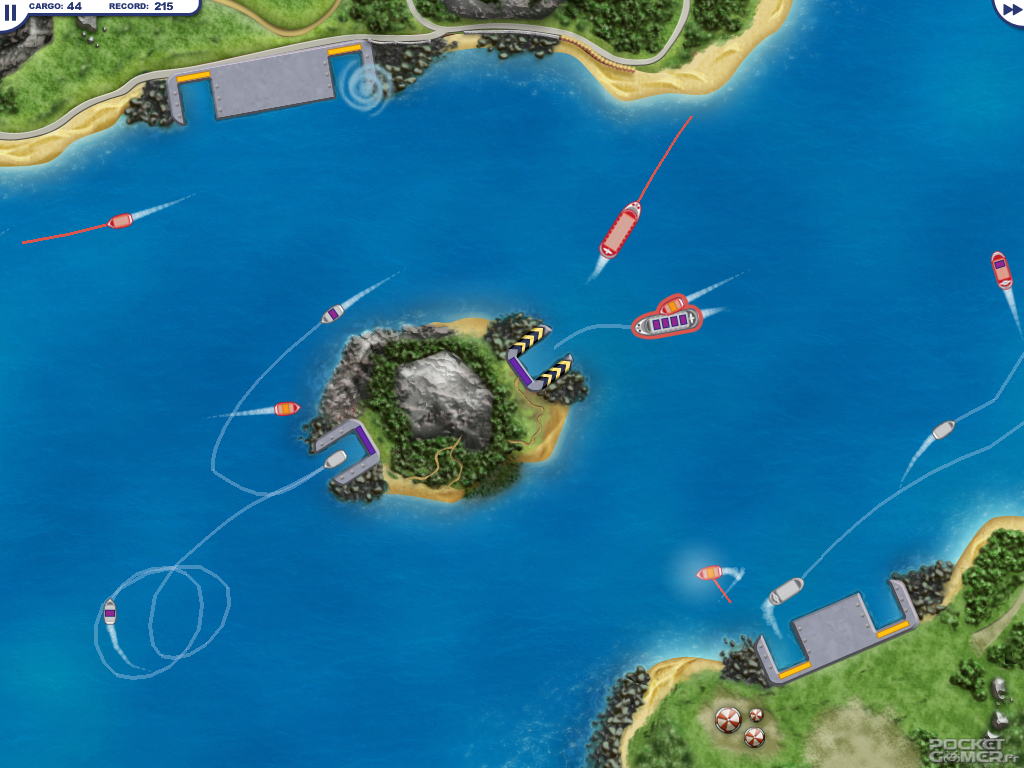
\includegraphics[width=\textwidth]{./images/harborMasterOriginal.png}
  \caption{Image du jeu original}
  \label{fig:harborMasterOriginal}
\end{figure}

Voilà comment se présente le jeu original (figure~\ref{fig:harborMasterOriginal}). N'ayant pas à nous attarder sur le graphisme du jeu, nous représenterons les bateaux par des formes simples selon leur type (carrés, cercles), et de même pour les ports. Une maquette est disponible en figure~\ref{fig:maquette}, l'aspect graphique définitif pourra différer. 


\begin{figure}[h]
	\begin{center}
		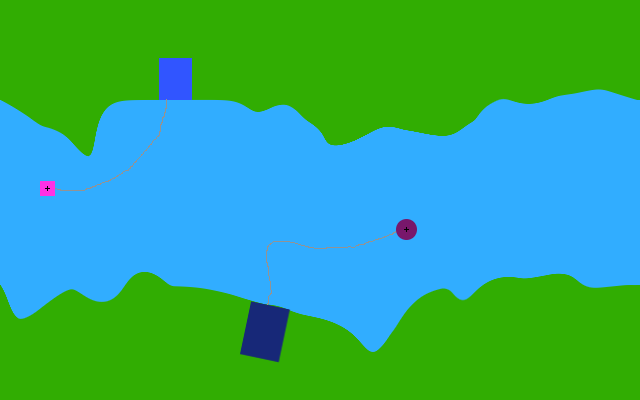
\includegraphics[width=\textwidth]{images/maquette}
	\end{center}
	\caption{Maquette de l'interface}
	\label{fig:maquette}
\end{figure}




~\newpage ~
\pageQuatriemeCouverture{}

\end{document}



